\documentclass{anstrans}
%%%%%%%%%%%%%%%%%%%%%%%%%%%%%%%%%%%
\title{Preliminary Design of an HGTR Micro-Reactor for Site Evaluation}
\author{Zo{\"e} Richter,$^{*}$ Kathryn Huff,$^{\dagger}$}

\institute{
$^{*}$Advanced Reactors and Fuel Cycles, University of Illinois at Urbana-Champaign, Department of Nuclear, Plasma, and Radiological Engineering,
Urbana-Champaign, IL, zrichte2@illinois.edu
\and
$^{\dagger}$Assistant Professor,University of Illinois at Urbana-Champaign, Department of Nuclear, Plasma, and Radiological Engineering , Urbana-Champaign, IL, 118 Talbot Laboratory, kdhuff@illinois.edu
}

%%%% packages and definitions (optional)
\usepackage{graphicx} % allows inclusion of graphics
\usepackage{booktabs} % nice rules (thick lines) for tables
\usepackage{microtype} % improves typography for PDF
\usepackage{float}

\newcommand{\SN}{S$_N$}
\renewcommand{\vec}[1]{\bm{#1}} %vector is bold italic
\newcommand{\vd}{\bm{\cdot}} % slightly bold vector dot
\newcommand{\grad}{\vec{\nabla}} % gradient
\newcommand{\ud}{\mathop{}\!\mathrm{d}} % upright derivative symbol

\begin{document}
%%%%%%%%%%%%%%%%%%%%%%%%%%%%%%%%%%%%%%%%%%%%%%%%%%%%%%%%%%%%%%%%%%%%%%%%%%%%%%%%
\section{Introduction}
As generation III reactors grow older, the nuclear industry looks ahead to the next generation of advanced reactor designs.  Generation IV has a wide breadth of designs, such as high-temperature gas-cooled reactors (HGTRs), molten salt reactors, or metal-cooled designs.  In addition to modernized geometries, fuel forms, and materials, some designs have scaled down, targeting remote locations and small installations in need of a power source that is stable and low-capacity.

The new generation brings new regulatory challenges, however.  Most designs aren't truly comparable to LWRs, especially when the fuel form changes, in the case of TRISO or liquid fuels.
The NRC released guidance in 2019 \cite{nrc_staff_population-related_2019} to foster discussion of new reactor siting regulations.  In this report, four options were identified: site all new reactors under the same LWR guidelines, site reactors based on their source term, site based on their source term and expected accident scenarios, and to site each reactor on a case-by-case basis.

Option 1 is grossly inaccurate, while option 4 would require such a great change in regulatory guidelines and extra work that cost becomes prohibitive.

With this in mind, a 20 MWth gas-cooled micro-reactor inspired by the Xe-100 design has been created to support NRC regulation of such small reactors.  The presented work will examine the expected isotopic inventory overtime, and compare the accuracy of tracking the history of individual pebbles versus a more homogenized method.

%%%%%%%%%%%%%%%%%%%%%%%%%%%%%%%%%%%%%%%%%%%%%%%%%%%%%%%%%%%%%%%%%%%%%%%%%%%%%%%%
\section{Theory}
The second option regulatory option determines societal risk, SR, based on the expected dose to the surrounding population in the case of an accident.  SR is defined as:
\begin{subequations} \label{eqs:NRCSR}
\begin{equation} \label{eq:SRspecific}
SR = \pi r^{2} * D * ppsm
\end{equation}
\end{subequations}
Where r is the radial distance from the reactor boundary, D is the source term, and ppsm is the population density.  This allows for a simplified assessment and comparison between reactors with a source term significantly different from an LWR, such as a small-modular or micro-reactor.

The proposed reactor is a 20 MWth helium-cooled TRISO-pebble bed reactor, using 19.75\% uranium oxycarbide as the kernel in the TRISO particles.  An initial model looks at a slightly larger 200 MWth design at a lower enrichment of 15.5\% to use as a starting point for the final scale-down.
\begin{figure}[H]
  \centering
  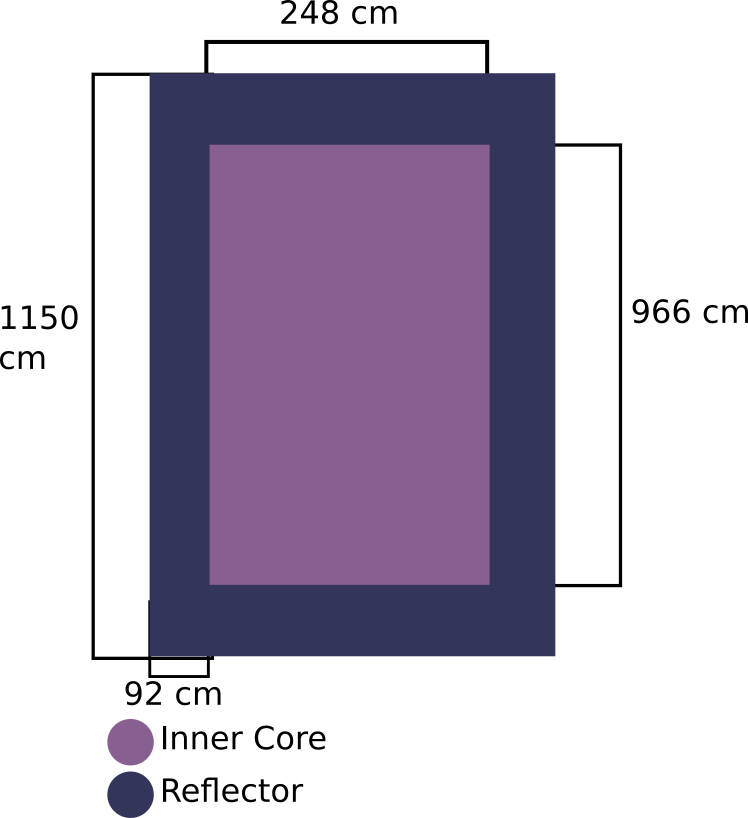
\includegraphics[width = \linewidth]{reactor-geom}
  \caption{Dimensions of the core barrel, in cm (not to scale)}
  \label{fig:voltage}
\end{figure}

The pebbles are assumed to take six passes through the core, each one taking six months.  Adding in the fresh fuel blend, this gives seven possible isotopic compositions.  The compositions of the burned pebbles are found using a single pebble model of a fresh pebble, burned in six six-month increments.

\begin{table}[H]
  \centering
  \caption{Fuel Cycle Analysis Methods}
  	\begin{tabular}{cc}\toprule
 		& Depletion Time [Days]\\
 		\midrule
 		Fuel-0 (fresh) & 0 \\
 		Fuel-1 & 180 \\
 		Fuel-2 & 360 \\
 		Fuel-3 & 541 \\
 		Fuel-4 & 720 \\
 		Fuel-5 & 900 \\
 		Fuel-6 & 1080 \\
	\bottomrule
	\end{tabular}
  \label{tab:fueltypes}
\end{table}

In order to determine the level of detail needed to accurately assess the reactor's source term - and consequently, the societal risk, three methods of handling the pebbles are proposed.

\begin{table}[H]
  \centering
  \caption{Fuel Cycle Analysis Methods}
  	\begin{tabular}{ccc}\toprule
 		& \# of Fuel Compositions & \# of Core Sections \\ \midrule
 		Method A & 1 & 1 \\
 		Method B & 7 & 1 \\
 		Method C & 7 & 6 \\
	\bottomrule
	\end{tabular}
  \label{tab:fuelcycles}
\end{table}

\subsection{Method A}
The simplest method averages the seven compositions by mass fraction into one homogenous fuel type.  This is distributed in all pebbles, which are randomly distributed throughout the active core using the random particle dispersal utility in Serpent 2.
\subsection{Method B}
Method B builds on A, replacing the wholly uniform blend with 7 unique compositions, each randomly distributed throughout the core volume using the same dispersal routine.  This method better tracks the history of the pebbles, at the cost of added complexity.
\subsection{Method C}
The final, highest fidelity model uses the same initial fuel blends as B, but splits the core into six, equal axial layers.  This is to better simulate the change in composition as the pebbles travel down through the core.
For the movement of each layer, it is assumed that the pebbles move in a slug-flow pattern \cite{cisneros_pebble_2013}, i.e. the pebbles in one section to not move relative to each other.  A full-core depletion model will be run for one month.  At this time, the layers each shift down one layer.  The bottom layer, which would leave the core, has the pebbles that are the most burned, Fuel-6, are replaced with Fuel-0 to simulate online refueling.  Then this ejected layer goes back into the space vacated by the previous top layer, and a new depletion calculation is run on this new core layout.  This is repeated until an equilibrium core state is reached.

% create a figure to place here that shows the fuel shuffling in a compact way

%%%%%%%%%%%%%%%%%%%%%%%%%%%%%%%%%%%%%%%%%%%%%%%%%%%%%%%%%%%%%%%%%%%%%%%%%%%%%%%%
\subsection{Full Core Model}

The initial core model is given below, with pebbles distributed in one section as in methods A and B

\begin{figure}[H]
  \centering
  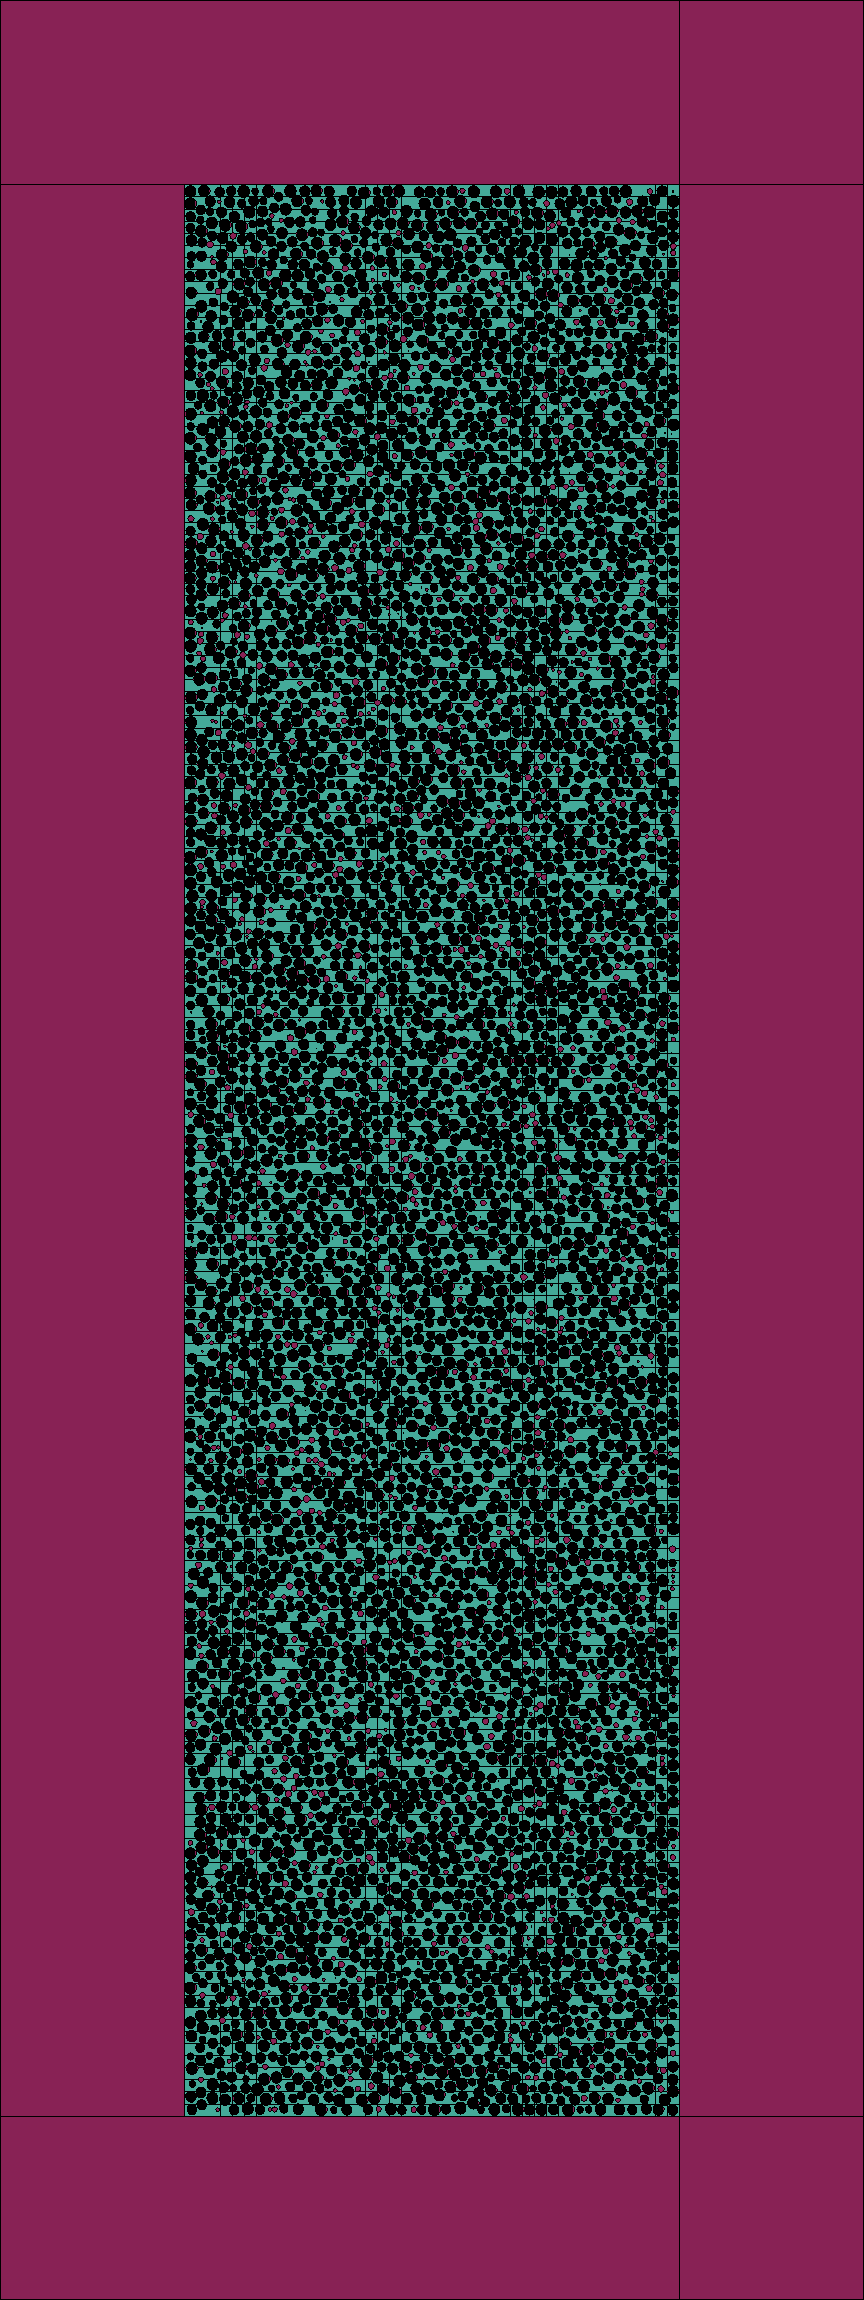
\includegraphics[width = \linewidth]{htgr-mr-full-core-axial}
  \caption{Cross-section of the core barrel through the yz plane}
  \label{fig:axial-xs}
\end{figure}

\begin{figure}[H]
  \centering
  \includegraphics[width = \linewidth]{htgr-mr-full-core-radial}
  \caption{Cross-section of the core-barrel through the xy plane}
  \label{fig:radial-xs}
\end{figure}

While this current model has individual TRISO particles modeled \ref{fig:radial-zoom}, moving forward, especially as Method C is examined in more detail, the pebbles will be homogenized into one uniform material.

\begin{figure}[H]
  \centering
  \includegraphics[width = \linewidth]{htgr-mr-close-up}
  \caption{Closer look at the pebble layout, cut throught the xy plane at the center}
  \label{fig:radial-zoom}
\end{figure}

%%%%%%%%%%%%%%%%%%%%%%%%%%%%%%%%%%%%%%%%%%%%%%%%%%%%%%%%%%%%%%%%%%%%%%%%%%%%%%%%
\section{Results}

The inital full core model shows that the region with the highest rate of fission is centered in the core \ref{fig:axial-fission-scatter}.  This peak region is expected to shift upwards in Method C, when the fuel distribution varies axially.

\begin{figure}[H]
  \centering
  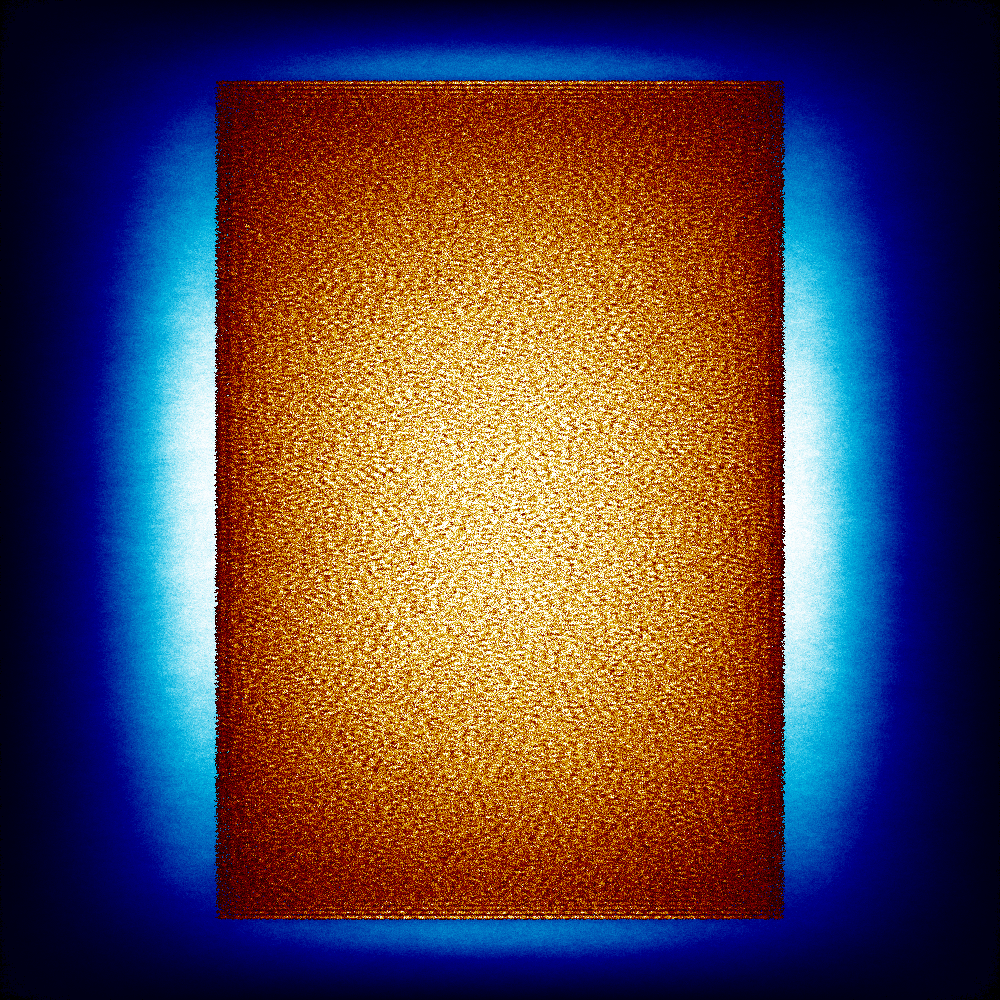
\includegraphics[width = \linewidth]{htgr-mr-full-core-radial-mesh}
  \caption{Fission and scattering rate in an axial cross section of the core}
  \label{fig:axial-fission-scatter}
\end{figure}

The inital depletion of a fresh 15.5\% enriched pebble showed a final cumulative burnup of 118.8 MWd/kgU.  This is of course expected to change when the enrichment increases and the geometry changes in the scaled-down model.

%%%%%%%%%%%%%%%%%%%%%%%%%%%%%%%%%%%%%%%%%%%%%%%%%%%%%%%%%%%%%%%%%%%%%%%%%%%%%%%%


%%%%%%%%%%%%%%%%%%%%%%%%%%%%%%%%%%%%%%%%%%%%%%%%%%%%%%%%%%%%%%%%%%%%%%%%%%%%%%%%
\section{Conclusions}


%%%%%%%%%%%%%%%%%%%%%%%%%%%%%%%%%%%%%%%%%%%%%%%%%%%%%%%%%%%%%%%%%%%%%%%%%%%%%%%%
\appendix
\section{Appendix}


%%%%%%%%%%%%%%%%%%%%%%%%%%%%%%%%%%%%%%%%%%%%%%%%%%%%%%%%%%%%%%%%%%%%%%%%%%%%%%%%
\section{Acknowledgments}
This research is funded by the Nuclear Regulatory Commission.

The author would like to thank the other members of the Advanced Reactors and Fuel Cycles group at the University of Illinois at Urbana-Champaign

%%%%%%%%%%%%%%%%%%%%%%%%%%%%%%%%%%%%%%%%%%%%%%%%%%%%%%%%%%%%%%%%%%%%%%%%%%%%%%%%
\bibliographystyle{ans}
\bibliography{2020-richter-ans-winter.bib}
\end{document}

